\documentclass[a4paper,openright, 14pt]{article}
\usepackage[utf8]{inputenc}
\usepackage{graphicx}
\usepackage{amsmath}
\usepackage{tikz}
\usetikzlibrary{datavisualization}
\usetikzlibrary{datavisualization.formats.functions}

\graphicspath{ {./images/} }

\usepackage{fullpage}
\newcommand{\ssection}[1]{%
\section[#1]{\centering\normalfont\scshape #1}}
\newcommand{\ssubsection}[1]{%
\subsection[#1]{\bfseries\normalfont\scshape #1}}
\newcommand{\ssubsubsection}[1]{%
\ssubsubsection[#1]{\bfseries\normalfont\scshape #1}}

\title{Third and Final Study Guide}
\author{The LAJendary Crew}
\date{May 2019}

\begin{document}

\maketitle
\underline{\section*{{Taylor and Maclaurin Series}}}
\subsection*{Introduction}
\\Question: how would we be able to approximate a value of a function with out substituting numbers into it?
\\\\
Answer: As we learned in Calculus AB we can use a linear tangent line to help us. However what if we could take it a step further. Let's us use a polynomial to help us solve for a specific value. For example let's start with a simple quadratic, $y=x^2 +x+1$. First try to create a line in which the first derivative and the function are both the same for our polynomial and our new one at $x=0$.
$$y(0)=x^2 +x +1$$
$$T_1 (x)= ax +b$$
Function value at x=0.\\
Now in order to get the first two derivatives of both functions to equal each other we first have to derive each term.
\begin{align*}
 f(x)&=x^2  + x+1    &    T_1(x)&=ax^2 +bx +c       \\
f'(x)&=2x+1    &    T_1 '(x)&=2ax +b       \\
f''(x)&=2    &    T_1 ''(x)&=2a   
\end{align*}
Now as shown before find $f(0)$ and $T_1 (0)$ and then set them equal to each other. Then do the same for their following derivatives.
\begin{align*}
 f(0)&=(0)^2  + (0)+1 = 1   &    T_1(0)&=a(0)^2 +b(0) +c = c      \\
f'(0)&=2(0)+1 =1  &    T_1 '(0)&=2a(0) +b   = b    \\
f''(0)&=2    &    T_1 ''(0)&=2a 
\end{align*}

$$a=1$$
$$b=1$$
$$c=1$$
\\ So...
$$T_1(x)= x^2 +x +1$$
\\
Notice how we will always end up with the same polynomial when we use a polynomial to find another. Polynomials will always be approximated by themselves with this process because we are using them.
\\\\
Continuing on, this is a formula for this process that we just did which applies to all functions. It is called the Taylor Series.
$$\sum_{n=0} ^\infty \frac{f^n(x_0)}{n!} (x-x_0)^n$$
\\
Let's examine what each part is and what it does.\\\\
-First we shall examine what $f^n(x_0)$ means. $f(x)$ is the function. The $^n$ part of it means the derivatives of the function. Example: when $f^1(x_0 )$ that means $x_0$ is being evaluated at the first derivative of $f(x)$ ,$f'(x_0)$. $f^0 (x)$ is just $f(x)$. $x_0$ is the center or the point at which we will set our function equal to. *A Maclaurin Series is centered at $x=0$ or $(x_0 -0)$. Lastly $f^n (x_0)$ will always be a constant. \\\\
-Second $x_0$ is not only used with the functions but it is also put into inside the parentheses of the polynomial generator $(x-x_0)^n$ which will give us a higher degree polynomial for every term used.\\\\
-Lastly the reason for Everything for being divided by $n!$ is because we every time we derive $a\cdot x^n$, where a is a constant we would end up with a number of $n! \cdot a$. To eliminate the factorial to isolate the constant a we would need to divide it all by $n!$.
for example we will use the Taylor series in an example. We first need a function like this $$f(x)=x^3+2x^2+3x+3$$ and we will center it around $x=0$ (a Maclaurin series) which means our first term will be $\frac{f(0)(x-0)^0}{0!}$ and the second will be $\frac{f'(0)(x-0)^1}{1!}$ and the third will be $\frac{f"(0)(x-0)^2}{2!}$ the fourth is $\frac{f"'(0)(x-0)^3}{3!}$.
$f(0)=3$ , $f'(0)=3$ , $f"(0)=4$ ,and $f"'(0)=6$ and anything after is just 0, so now we can write the series out to look like $$3+3x+2x^2+x^3$$ We see how it came out with the same function. So we see that it can be used to approximate a function and if only go up to the first few terms you can usually get a good approximation. It built a function out of function, but some functions aren't easy, because they aren't in the form of a usable function with so Taylor series' can be used to make an easy function to use. Here's a pic of each term approaching the function value.
\begin{center}
    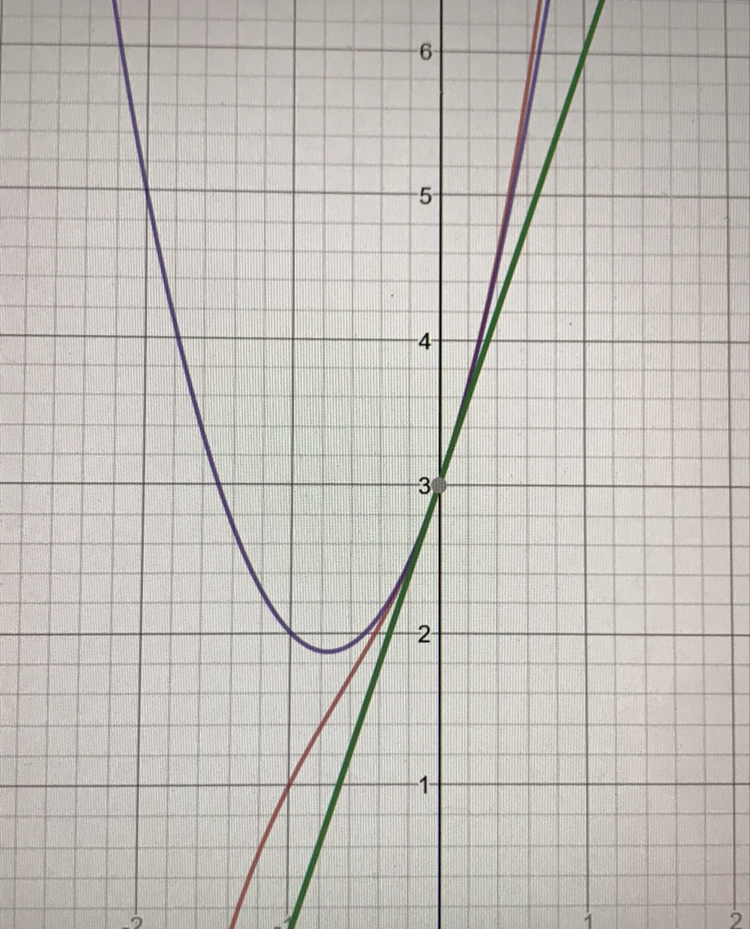
\includegraphics[width = 5cm, height = 5cm ]{graph.jpeg}
\end{center}
\subsection*{Series of Familiar Functions}
    There are some functions that show up a lot which create series that are easy to use and good to remember because they can easily be manipulated to create other series' and solve functions. The series' that we will will talk about are made from the functions of $sin(x), cos(x), e^x, \frac{1}{1+x}, \frac{1}{1-x}$ and $ln(1+x)$. With these we are going to use Maclaurin series'. we will build a function for $f(x)=sin(x)$ from scratch. This one is one of the ones that you can't just substitute numbers it, we will have to build a function. The first term will be $\frac{f(0)(x)^0}{0!}$ and the second will be $\frac{f'(0)(x)^1}{1!}$ and the third will be $\frac{f"(0)(x)^2}{2!}$ the fourth is $\frac{f"'(0)(x)^3}{3!}$....and so on $\frac{f^n(0)(x)^n}{n!}$
\\$f(0)=sin(0)=0$, $f'(0)=cos(0)=1$, $f"(0)=-sin(0)=0$,and $f"'(0)=-cos(0)...$ repeating the same pattern of $0,1,0,-1$ which makes the function of $0+1(x)+0(x^2)-\frac{x^3}{3!}....$ which is $$x-\frac{x^3}{3!}+\frac{x^5}{5!}...\frac{(-1)^nx^{2n+1}}{{(2n+1)}!}$$ we also see that these are series that can be modeled with the general term as a sum $$\sum_{n=0} ^\infty \frac{(-1)^n(x)^{2n+1}}{(2n+1)!}$$ and that is the Maclaurin of sin(x). Here is a pic as the terms approach the function \begin{center}
    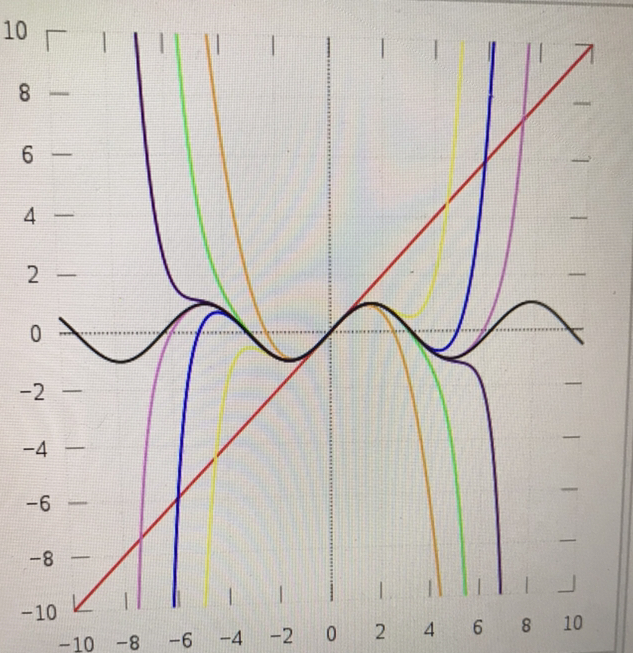
\includegraphics[width = 5cm, height = 5 cm]{sin.jpeg}
\end{center}
The series of cos(x) is similar because it is the derivative of sin so it ends being the derivative of sin's series and looks likes this. $$1-\frac{x^2}{2!}+\frac{x^4}{4!}...\frac{(-1)^nx^{2n}}{(2n)!}$$ and the sum is $$\sum_{n=0} ^\infty \frac{(-1)^n(x)^{2n}}{(2n)!}$$
\\ Another couple of series that we will look at are $\frac{1}{1+x}$ and $\frac{1}{1-x}$ the series of the latter looks like this when put into the formula The first term will be $\frac{f(0)(x)^0}{0!}$ and the second will be $\frac{f'(0)(x)^1}{1!}$ and the third will be $\frac{f"(0)(x)^2}{2!}$ the fourth is $\frac{f"'(0)(x)^3}{3!}$....and so on $\frac{f^n(0)(x)^n}{n!}$ 
$f(0)=1$, $f'(0)=1$, $f"(0)=2$, and $f"'(0)=6$ which is $$1+x+\frac{2x^2}{2!}+\frac{6x^2}{3!}+...\frac{n!x^n}{n!}$$ which is $$1+x+x^2+x^3...x^n$$  $$\sum_{n=0} ^\infty x^n$$ here is a pic of this graph 
\begin{center}
    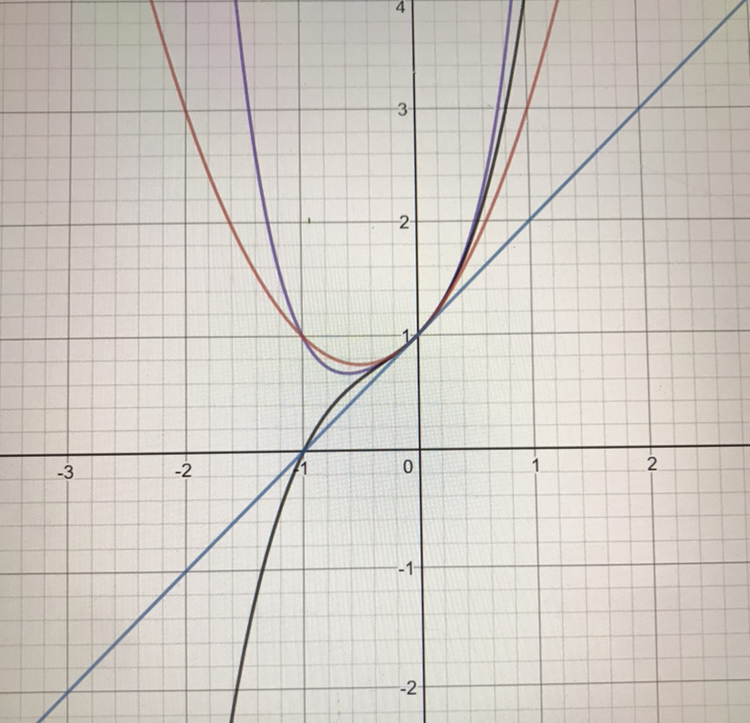
\includegraphics[width = 5cm, height = 5 cm]{imsotired.jpeg}
\end{center} 
its counterpart function $$\frac{1}{1+x}$$ has $f(0)=1$, $f'(0)=-1$, $f"(0)=2$, and $f"'(0)=-6$. We see this is very similar except that there are negative values every other term so the series would be $$1-x+x^2-x^3...(-1)^nx^n$$
and the series in sum form would be $$\sum_{n=0} ^\infty (-1)^nx^n$$. The last set of these equations are of $ln(1+x)$ and $e^x$ we will again start with the latter every derivative value of $e^x$ is $e^x$ and when $0$ is substituted in, it is 1 so it it the bare bones of a  Maclaurin series. That means we can just use the formula so we can start with the equation that we already know $$\sum_{n=0} ^\infty \frac{f^n(x_0)}{n!} (x)^n$$ and since any derivative of $e^x$ at 0 is 1 we can say that the sum is $$\sum_{n=0} ^\infty \frac{(x)^n}{n!}$$ and this forms the series $$1+x+\frac{x^2}{2!}+\frac{x^3}{3!}....\frac{x^n}{n!}$$ for $ln(1+x)$ we will also see the derivatives are $f(0)=0$, $f'(0)=1$, $f"(0)=-1$, and $f"'(0)=2$ which forms the series
$$x-\frac{x^2}{2}+\frac{x^3}{3}...\frac{(-1)^nx^{n+1}}{n+1}$$ and it has the sum of $$\sum_{n=0} ^\infty.\frac{(-1)^nx^{n+1}}{n+1}$$. So these are all the equation you need for some series of these recurring functions. Lets test some of these out.
\underline{Example 1}
What is the fifth term in the Maclaurin sequence of $e^x$? So we just have to think about what $e^x$ is as a sum which is $$\sum_{n=0} ^\infty \frac{(x)^n}{n!}$$ and forms the sequence $$1+x+\frac{x^2}{2!}+\frac{x^3}{3!}+\frac{x^4}{4!}$$ and that last term is the fifth term.
\underline{Example 2} write out the first four terms of sin(x).
Like the last one we need to find the sum which is $$\sum_{n=0} ^\infty \frac{(-1)^n(x)^{2n+1}}{(2n+1)!}$$ and forms the series 
$$x-\frac{x^3}{3!}+\frac{x^5}{5!}-\frac{x^7}{7!}$$ and there you are the first four terms of the series.
\underline{Example 3} What is the fourteenth term of $\frac{1}{1-x}$? The series is modeled by $$\sum_{n=0} ^\infty x^n$$ and the fourteenth term is when $n=13$ because 0 is also included so that means that the fourteenth term is $x^13$
\subsection*{Intervals of Convergence}
The interval of convergence holds true to its name: it's an interval of values where the series converges. There are three options for the bounds of convergence: all real numbers, 1 value (the center), or most commonly, a finite set. When we have a finite set, we also have a radius of convergence. The radius is the absolute value of the difference from the upper bound to the center and the lower bound to the center. In this way (much like a detective) we can use the bounds of convergence and the center to find the radius of convergence and the center. Before we move on, an example of a finite bound of convergence could be:
$$(-2,2)$$
In this case, 0 would be the center since the absolute value of the difference between -2 and 0 is 2, and the difference between 0 and 2 is 2. This "common difference", or 2, would be the radius of convergence.
\\
When the interval of convergence is all real numbers, there's still a radius of convergence and a center. In this case, the center would be 0 and the radius would be $\infty$.\\\\
So, how do we find intervals of convergence? We use the ratio test to find the bounds and check the bounds to see if they converge at the endpoints themselves. Let's try an example\\\\
\underline{Example 1}\\\\
Find the interval and radius of convergence. 
$$\sum\limits_{n=1}^{\infty} \frac{(x-3)^n}{n+2}$$
Let's start off by using the ratio test
$$\lim_{n\to\infty} |\frac{(x-3)^{n+1}}{n+3}\cdot \frac{n+2}{(x-3)^n}|$$
Which we can rewrite to be
$$|\frac{(x-3)^n(x-3)}{n+3} \cdot \frac{n+2}{(x-3)^n}|$$
As n approaches infinity, the limit of n+2 over n+3 will just approach 1, so we can cancel out these two terms. We can cross-multiply and cancel out the $(x-3)^n$. We’re left with
$$|x-3|$$
Since this is the ratio test, for it to converge this must be less than 1.
$$|x-3|<1$$
Let’s solve for the bounds\\
$x-3<1$ and $x-3>-1$
$x<4$ and $x>2$
Now we have to check the bounds and see if it converges there too. 
When x=4, the series is 
$$\sum\limits_{n=1}^{\infty} \frac{1}{n+2}$$
This series is the harmonic series, which we know diverges. So, 4 is not included in the interval of convergence.
When x=2, the series is
$$\sum\limits_{n=1}^{\infty} \frac{(-1)^n}{n+2}$$
This is the alternating harmonic series which we know converges conditionally.
So our bounds end up being $[2,4)$ where the radius is 1.\\\\
\underline{Example 2}\\\\
Find the interval and radius of convergence.
$$\sum\limits_{n=1}^{\infty} \frac{(2x+4)^n}{n!}$$
Use the ratio test
$$\lim_{n\to\infty}|\frac{(2x+4)^n(2x+4)}{(n+1)n!} \cdot \frac{n!}{2x+4}|$$
Simplify and we’re left with
$$|\frac{2x+4}{n+1}|<1$$
Since n is approaching infinity, the denominator will grow larger and larger, no matter the value of x. Therefore, any value of x will make the fraction smaller than one, making all real numbers possible. Our interval of convergence would look like this
$(-\infty, \infty)$ with our radius being $\infty$\\\\
\underline{Example 3}\\\\
Find the interval and radius of convergence.
$$\sum\limits_{n=1}^{\infty} n!(x+7)^n$$
Use the ratio test
$$\lim_{n\to\infty}|\frac{(n+1)n!(x+7)^n(x+7)}{n!(x+7)^n}$$
Simplify
$$\lim_{n\to\infty}|(n+1)(x+7)|<1$$
If we think about it, as n approaches infinity, this is only going to grow larger. So, the only value that we could possibly get less than one would be when infinity is multiplied by 0. For this to happen 
$$x+7=0$$
so x is -7. This sole value is the interval of convergence. Since there’s no difference in points because there’s only one value of convergence, the radius of convergence is 0.
\subsection*{Error: Alternating Series}
Let's begin. Simple task, find the error bound of an alternating series. First we must know if the Alternating series converges or not. In order to know this it must pass Absolute Convergence or Conditional Convergence, in which all the alternating terms lead to zero and decrease in absolute value every time. To explain this process easily, let's look at the alternating harmonic series which converges to $ln(2)$.
$$\sum_{n=1} ^{\infty} \frac{(-1)^{n+1}}{n}$$
Now let's use the actual value of the series and each time add a term to the series starting at the first term.
$$ln(2)\approx 0.693147$$
$$\sum_{n=1} ^1 \frac{(-1)^{n+1}}{n}=1$$
$$\sum_{n=1} ^2 \frac{(-1)^{n+1}}{n}=1-1/2=1/2$$
$$\sum_{n=1} ^3 \frac{(-1)^{n+1}}{n}=1-1/2+1/3\approx.8333$$
$$\sum_{n=1} ^4 \frac{(-1)^{n+1}}{n}=1-1/2+1/3-1/4\approx.58333$$
Notice how with each step we make the approximation has less of a margin for error compared to the actual value. Graph below to show comparison with each step...\\\\
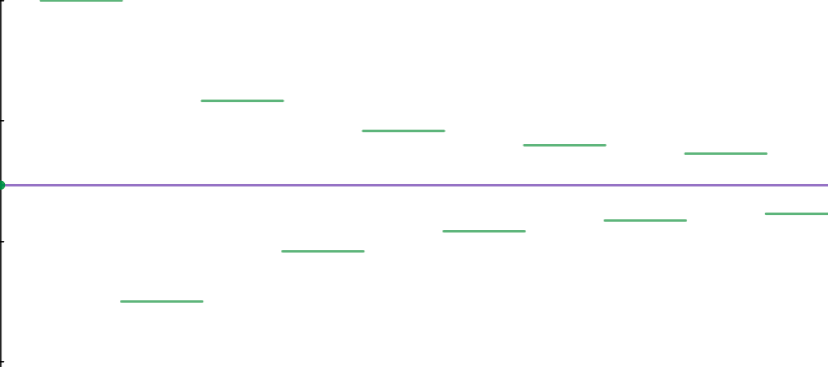
\includegraphics[width = 15cm, height = 3 cm]{fml.png}
\\
*Purple line represents the value of $ln(2)$\\\\

This absolute distance between the actual and each approximation is called the error bound. Now let's see if there is a pattern to this since we get smaller every time from the actual value. First, lets look at the absolute value of distance between the real value and each approximation starting at the first term.
$$|ln(2)-1|\approx0.30685281944$$
$$|ln(2)-1/2|\approx0.19314718056$$
$$|ln(2)-.83333|\approx 0.140186152773$$
$$|ln(2)-.58333|\approx 0.109813847227$$
\\\\
One pattern is primarily constant between each error of the series. The absolute value of the first omitted term, which is the term after the the amount of terms used, is larger than the absolute value of the error created using the other terms subtracting from the actual value. So...
\\
$$|S-S_n|\leq|a_{n+1} |$$
\\
*$S$ is actual sum value 
*$S_n$ is partial sum value 
*$a_{n+1}$ is the first omitted term.\\\\

This formula applies to all alternating series that converge to a finite value.\\\\

Now how does this relate to Taylor series anyways? Well, glad you asked. Say if we have a Maclaurin Series using the function $\cos{x}$ where the radius of convergence is all real numbers and we want to approximate the value of $\cos{1}$ within $\frac{1}{1000}$ of the actual value, How many terms would we use. We would first have to set up the Maclaurin series for $\cos{x}$ at $x=1$
$$\sum _{n=0} ^\infty  \frac{(-1)^n \cdot (x)^{2n}}{(2n)!}$$
all right substitute 1 for x.
$$\sum _{n=0} ^\infty  \frac{(-1)^n \cdot (1)^{2n}}{(2n)!}$$
$$\sum _{n=0} ^\infty  \frac{(-1)^n }{(2n)!}$$
Now see have we have created a new alternating series. Let's continue and find out which absolute valued partial sum gets us less than $\frac{1}{1000}$ from the actual value. To do this find the value of each term until absolute value of a term is less than one one-thousandth. We know that $6!$ is equal to 720, and we must go by $2n!$, so $8!$ is greater than 1000 and the term with it in its denominator will be our first omitted term. So..
$$|S-S_3|\leq|a_{4} |$$
$$|S-S_3|\leq|1/8! |<\frac{1}{1000}$$

Continuing this method will work even if their is no value in the input of the function. So you could create polynomials that will estimate a value within a certain margin for error. However this alternating series error bound only works for Taylor series with an alternating sequence inside of it.
\\\\
\\\\
\underline{\section*{Power Series}}
\subsection{Introduction}
As we learned with Taylor series, we build a function with polynomials. The idea of building just polynomials not derived from functions is what a power series is. A basic formula for a power series is...
$$\sum_{n=0} ^\infty C_n (x-x_0)^n$$
Here, $C_n$ and $x_0$ are both constants, where $x_0$ is where the polynomial is centered. Here, $x$ is the variable, showing that power series are all functions of x. Although this may seem slightly different from series with numerical terms, the power series is just a way to create a generalized term for a series. This generalized term makes it much easier to perform different functions on the series such as finding the derivative, integrating, or manipulating known series to create new ones. This process of having a generalized term with a variable of x allows for much quicker calculations, since we don't have to write out each individual term to find the derivative or manipulate a series. Let's see this for ourselves.
\subsection{Substitution}\\\\
Sometimes, we may be faced with a problem that we would have difficulty solving and need a strategy to solve it. Or, we may be forced to create a series that would be difficult to do without our knowledge of known Maclaurin series. We can now take this knowledge and use it to find a solution to a challenging problem, or create a series. Let's see this strategy tried out below.\\\\
\underline{Example 1}\\
Find a Maclaurin series for $1+xe^{x^2}$. Let's use our knowledge of the series for $e^x$ to solve this.
$$e^x=\sum _{n=0}^\infty \frac{x^n}{n!}=1+x+\frac{x^2}{2!} +...+\frac{x^n}{n!}+...$$
Whenever we do substitution, we'll always first want to deal with substituting in the new exponent of $e^x$ before moving on to other steps. This allows our answer to be accurate. Let's substitute $x^2$ in for $x$.
$$e^{x^2}=\sum _{n=0}^\infty \frac{x^{2n}}{n!}=1+x^2+\frac{x^4}{2!} +...+\frac{x^{2n}}{n!}+...$$
Now let's multiply $e^{x^2}$ by x since it's the operation that's closest to the function.
$$xe^{x^2}=\sum _{n=0}^\infty \frac{x^{2n}}{n!}\cdot x=\sum _{n=0}^\infty \frac{x^{2n+1}}{n!}=1+x^3+\frac{x^5}{2!} +...+\frac{x^{2n+1}}{n!}+...$$
Now, let's do the last step to finally get our manipulated series.
$$1+xe^{x^2}=1+ \sum _{n=0}^\infty \frac{x^{2n+1}}{n!}=2+x^3+\frac{x^5}{2!} +...+\frac{x^{2n+1}}{n!}+...$$
\underline{Example 2}\\\\
We have learned that $\lim_{x\to0} \frac{sinx}{x}$ is 1, but we don't know why. Now, we can use substitution of a known series to find this limit with proof that it works.\\\\
Find $\lim_{x\to0} \frac{sinx}{x}$ using series.
$$sinx=\sum _{n=0}^\infty \frac{(-1)^nx^{2n+1}}{(2n+1)!}=x-\frac{x^3}{3!}+\frac{x^5}{5!}...$$
$$\frac{sinx}{x}=\sum _{n=0}^\infty \frac{(-1)^nx^{2n}}{(2n+1)!}=1-\frac{x^2}{3!}+\frac{x^4}{5!}...$$
Now let's think about each term as x approaches 0.
$$\lim_{x\to0} \frac{sinx}{x}=1-\frac{0^2}{3!}+\frac{0^4}{5!}...$$
If we think about it, as x approaches 0, the numerator for all of the terms except for 1 will be 0 so the fractions will just end up equalling 0, making our answer 0.\\\\
\underline{Example 3}\\\\
Our process may change a little bit when we have to multiply two know series together. Let's try multiplying the series of $sinx$ and $e^x$ together to see what our answer is.\\\\
Find the first 3 non-zero terms of the series $e^xsinx$\\
Let's start by listing the first three terms of each series and writing them as a polynomial multiplied by the polynomial of the other series. This will allow us to easily multiply and identify our first 3 terms.
$$(1+\frac{x}{1}+\frac{x^2}{2})(x-\frac{x^3}{3!}+\frac{x^5}{5!})$$
If we think about it, the first (lowest) term that we can have is x (when 1 is multiplied by x). There can only be one x after multiplication so our first term is x. Our next lowest multiplied out term could contain $x^2$, and we could only have one term of this (when x is multiplied by x). So, our second term is $x^2$. So far, we have:
$$x+x^2$$
Now, our next term would contain $x^3$. Once multiplied out, the polynomial will have 2 $x^3$ terms so we'll have to combine them to create one. When multiplying $-\frac{x^3}{3!}$ by 1, we get $-\frac{x^3}{3!}$, or $-\frac{x^3}{6}$. After multiplying $\frac{x^2}{2!}$ by x, we get $\frac{x^3}{2}$. Let's simplify.
$$\frac{x^3}{2}-\frac{x^3}{6}=\frac{3x^3}{6}-\frac{x^3}{6}=\frac{2x^3}{6}=\frac{x^3}{3}$$
Therefore, our final polynomial is:
$$x+x^2+\frac{x^3}{3}$$
\subsection{Differentiation}
The Power series is always going to generate a massive polynomial every time we use it. We can easily derive these terms and always find the next derivative just by deriving again. Now, there is two ways for finding the derivative of the power series. We can derive the series in total using a couple of its terms and finding a pattern or derive the general term using the rules we know. To this, let's use the Maclaurin series of $e^x$ because when you derive $e^x$, it's derivative is just $e^x$.
$$\sum _{n=0}^\infty \frac{x^n}{n!}=1+x+\frac{x^2}{2!} +...+\frac{x^n}{n!}+...$$
$$ \frac{d}{dx}(\sum _{n=0}^\infty\frac{x^n}{n!})= 0+1+\frac{2\cdot x}{2!} +\frac{3\cdot x^2}{3!}+ ...$$
$$ \frac{d}{dx}(\sum _{n=0}^\infty\frac{x^n}{n!})=1+x+\frac{x^2}{2!} +...+\frac{x^n}{n!}+...$$
Same pattern is formed so...
$$ \frac{d}{dx}(\sum _{n=0}^\infty\frac{x^n}{n!})=\sum _{n=0}^\infty \frac{x^n}{n!}$$
This is already proven because the derivative for $e^x $ is itself. Now let's do the same function but derive the general term using knowledge that we know.
$$ \frac{d}{dx}(\sum _{n=0}^\infty\frac{x^n}{n!})=\sum _{n=0}^\infty\frac{n \cdot x^{n-1}}{n \cdot (n-1)!}$$
$$ \frac{d}{dx}(\sum _{n=0}^\infty\frac{x^n}{n!})=\sum _{n=0}^\infty\frac{ x^{n-1}}{ (n-1)!}$$
The first term does not exist so we shall change the bounds. Then we will alter it by changing the bounds and the series again. 
$$\sum _{n=0}^\infty\frac{ x^{n-1}}{ (n-1)!}=\sum _{n=1}^\infty\frac{ x^{n-1}}{ (n-1)!}$$
$$\sum _{n=1}^\infty\frac{ x^{n-1}}{ (n-1)!}=\sum _{n=0}^\infty\frac{ x^{n-1+1}}{ (n-1+1)!}$$
$$\sum _{n=0}^\infty\frac{ x^{n-1+1}}{ (n-1+1)!}=\sum _{n=0}^\infty\frac{ x^{n}}{ (n)!}$$

Now we are back to where we began. Lastly, let's try one more Maclauren Series. Let's use $\sin{x}$ because its derivative is simply just $\cos{x}$.
$$\cos{x}=\sum _{n=0} ^\infty \frac{(-1)^n \cdot x^{2n+1}}{(2n+1)!}$$ 
$$\frac{d}{dx}(\sum _{n=0} ^\infty \frac{(-1)^n \cdot x^{2n+1}}{(2n+1)!})=\sum _{n=0} ^\infty \frac{(-1)^n (2n+1)\cdot x^{2n+1-1}}{(2n+1)!}$$ 
$$\sum _{n=0} ^\infty \frac{(-1)^n (2n+1)\cdot x^{2n}}{(2n+1)!}$$ 
$$\sum _{n=0} ^\infty \frac{(-1)^n x^{2n}}{(2n)!}=\cos{x}$$ 
This process will work for most if not all power series.
\\\\
\\\\
\subsection{Integration}
Integration of power series is exactly what it sounds like integrating series' and all of their terms. This is another way of manipulation of power series' to find other series from the familiar functions that we know as well as substitute other variables into it. It doesn't change the interval of convergence. Like any integral it takes the antiderivative of the function you are integrating. It can be both definite and indefinite integrals.
\\For 
\underline{Example 1} 
Lets just take the integral of cos(x) which has the sequence $$1-\frac{x^2}{2!}+\frac{x^4}{4!}...$$ the integral is 
$$ \int(cos(x))dx$$ which is just sin(x) and we know the series of that already which is $$x-\frac{x^3}{3!}+\frac{x^5}{5!}...$$ another way to solve these is by integrating each term of the series. like $$\int(1-\frac{x^2}{2!}+\frac{x^4}{4!})dx=x-\frac{x^3}{3!}+\frac{x^5}{5!}$$
So we can do these problems in different ways and they will come out to the same result.
\\\underline{Example 2}
In this example we will take the equation of $\frac{1}{x+1}$ and integrate it. If we take the normal integral of it we get $ln(|x+1|)$ which we know series for. We can also do it out like the other one where we know but we still solve it out anyway. The integral looks like this $$ \int(\frac{1}{x+1})dx=\int(1-x+x^2-x^3+x^4)dx$$ which equals $$ln(1+x)=x-\frac{x^2}{2}+\frac{x^3}{3}-\frac{x^4}{4}+\frac{x^5}{5}$$
Here is a pic of the graph
\begin{center}
    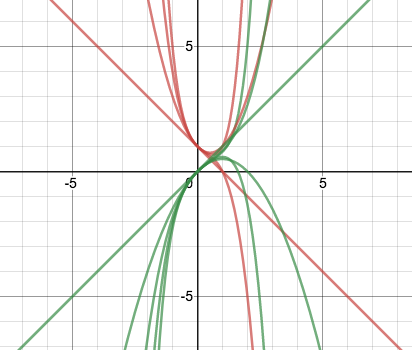
\includegraphics[width = 5cm, height = 5 cm]{ihatethis.png}
\end{center} 
The graphs of each one are shown here with the ones on bottom of $ln(|x+1|)$ and the ones on top of $\frac{1}{x+1}$
\\\underline{Example 3}
Our last example will be to integrate $e^x$ but
 with a twist this time using $e^t$ and integrating from 0 to x like this $$\int\limits_0 ^t(e^t)dt$$ which is $$\int\limits_0 ^t(1+t+\frac{t^2}{2!}+\frac{t^3}{3!})dt$$ which equals $$t+\frac{t^2}{2!}+\frac{t^3}{3!}+\frac{t^4}{4!}$$ from 0 to $x=$ $$x+\frac{x^2}{2!}+\frac{x^3}{3!}+\frac{x^4}{4!}$$ and that it because all terms have t and any substitutions would be 0 so you subtract 0 and it would be the same thing.
 \end{document}
